
\documentclass[a4paper,11pt]{article}
\usepackage[left=2cm, right=2cm, top=2cm]{geometry}
\usepackage{amsmath}
\usepackage{amsthm}
\usepackage{amssymb}
\usepackage{amsfonts}
\usepackage[colorlinks = true]{hyperref}
\usepackage{graphicx}
\usepackage{float}
\usepackage{needspace}
\usepackage{fancyhdr}
\usepackage{color,xcolor}
\usepackage{enumitem}
\usepackage{longtable,array,booktabs}
\usepackage{setspace}
\usepackage{xcolor}
\usepackage{xepersian}
\usepackage{mathtools}
\usepackage{flexisym}
\usepackage{fontspec}


\settextfont{XB Niloofar}
\setdigitfont{XB Niloofar}
\setlatintextfont{XB Niloofar}
\setmonofont{DejaVu Sans Mono}

\newcommand{\Code}[1]{\lr{\texttt{\detokenize{#1}}}}
\newcommand{\En}[1]{\lr{#1}}
\graphicspath{{figures/}{../figures/}}
\setstretch{1.19}
\setlength{\parindent}{0pt}\setlength{\emergencystretch}{2em}
\setlength{\parskip}{0.35em}
\renewcommand{\arraystretch}{1.23}
\hypersetup{hidelinks,pdfauthor={NACC Dataset C -- Statistics Course},pdftitle={Phase 1 NACC UDS and MRI}}
\begin{document}

\thispagestyle{fancy}
\fancyhf{}
\lhead{

 
\includegraphics[width=3cm]{logo.PNG}
 \vspace{-2pt}
}
\chead{\leavevmode{\Huge به نام خدا}\vspace{15pt}\\  {\Large علیرضا جنتی}\vspace{10pt}\\{\small 403101672}\vspace{5pt}}
\rhead{

  {\large   پروژه درس آمار}

\vspace{10pt}   

{\large  فاز اول}

\vspace{10pt}

ترم 14051
\vspace{-7pt}

}
\cfoot{\thepage}

\leavevmode
\vspace{20pt}


\vspace{1cm}

\begingroup
\hypersetup{linkcolor=blue}
\tableofcontents
\pagenumbering{gobble}
\endgroup
\clearpage
\pagenumbering{arabic} 
\pagebreak
\section{دامنه، سوال پژوهش و مبنای گزارش}
این گزارش فقط مربوط به فاز اول مسیر ج و زیرمجموعه تحویلی تیم درس از داده‌های \En{NACC} است.

\textbf{عنوان نهایی:} بررسی ارتباط شدت اختلال بالینی با میانگین ضخامت قشر انتورینال در زیرمجموعه \En{UDS--MRI} مرکز \En{NACC}.

\textbf{سوال اصلی نهایی:} در زیرمجموعه تحویلی \En{NACC}، چه ارتباط آماری‌ای میان نمره شدت اختلال بالینی \Code{CDRSUM} و میانگین ضخامت قشر انتورینال مغز در دو نیمکره وجود دارد و این ارتباط با درنظرگرفتن سن و جنس شرکت‌کنندگان چگونه تغییر می‌کند؟

\textbf{واحد تحلیل:} یک شرکت‌کننده با شناسه یکتای \Code{NACCID}. هر فایل تحویلی از هر فرد یک ردیف دارد؛ این موضوع، یکتایی مراجعه در پایگاه اصلی یا هم‌زمانی MRI و ارزیابی بالینی را ثابت نمی‌کند.


\subsection*{نقش متغیرها در سوال نهایی}
\small
\begin{longtable}{ p{4.9cm} p{4.9cm} p{5.0cm} }
\toprule
متغیر & مقیاس/منبع & نقش \\
\midrule
\endfirsthead
\toprule
متغیر & مقیاس/منبع & نقش \\
\midrule
\endhead
\Code{CDRSUM} & کمی گسسته / UDS & توضیحی اصلی (X): شدت بالینی \\
\Code{ENTORHINAL_MEAN_AVGTH} & کمی پیوسته / MRI مشتق‌شده & پاسخ اصلی (Y): میانگین ضخامت دوطرفه \\
\Code{NACCAGE} & کمی / UDS & توضیحی کمکی: سن \\
\Code{SEX} & طبقه‌ای / UDS & توضیحی کمکی: جنس \\
\Code{NACCUDSD} & طبقه‌ای / UDS & گروه‌بندی صرفا توصیفی \\
\Code{NACCID} & شناسه / هر دو & کلید اتصال؛ نه متغیر تحلیلی \\
\bottomrule
\end{longtable}
\normalsize
\textbf{فرضیه علمی اولیه:} انتظار می‌رود نمره‌های بالاتر \Code{CDRSUM} با میانگین ضخامت انتورینال پایین‌تر همراه باشند؛ این انتظار از پیش نتیجه تحلیل را تعیین نمی‌کند. نقش سن و جنس در این فاز صرفا معرفی می‌شود و بررسی آماری تعدیل‌شده به مراحل بعدی موکول است.

\section{منشا داده و سازوکار جمع‌آوری}
\En{NACC} داده‌های چندمرکزی مراکز پژوهش بیماری آلزایمر (\En{ADRC}) را نگه‌داری می‌کند.
\En{UDS} شامل اطلاعات جمعیت‌شناختی، وضعیت بالینی، عملکرد و شناخت است؛ داده MRI
از فرایند تصویربرداری و پردازش تصویری حاصل می‌شود. گردآوری ماهیت مشاهده‌ای
دارد و مداخله یا تخصیص تصادفی برای این پرسش انجام نشده است.
تاریخِ انجماد داده، بازه دقیق ورود نمونه به زیرمجموعه، روش ساخت آن و منشا پردازش ویژگی‌های MRI در CSVهای تحویلی مستند نشده‌اند.
برای شاخص‌های ضخامت، واحد \En{mm} بر پایه قرارداد رایج این نوع خروجی MRI نوشته شده.
\subsection*{فهرست و ابعاد فایل‌های تحویلی}
\small
\begin{longtable}{ p{9.0cm} r r }
\toprule
فایل/بخش & ردیف & ستون \\
\midrule
\endfirsthead
\toprule
فایل/بخش & ردیف & ستون \\
\midrule
\endhead
\Code{udslong_imputed.csv} & 1237 & 180 \\
\Code{mriscanclean.csv} & 1237 & 126 \\
\Code{combined_adjacency_matrix.csv} & 62 & 63 \\
\bottomrule
\end{longtable}
\normalsize

ماتریس مجاورت در CSV دارای ۶۲ ردیف و ۶۳ ستون شامل ستون برچسب است؛
بخش عددی آن ماتریسی \En{62 $\times$ 62} است.

\section{واحد مشاهده و ساختار داده}
در داده‌های طولی اصلی NACC ممکن است یک شرکت‌کننده چند مراجعه \En{UDS} داشته باشد.
اما هر یک از فایل‌های تحویلی \En{UDS} و \En{MRI} دقیقا 1237 ردیف و
1237 شناسه یکتا دارند. تعداد مراجعات واقعی هر فرد، شماره مراجعه انتخاب‌شده،
تاریخ معاینه و تاریخ اسکن در زیرمجموعه فعلی در دسترس نیستند؛ پس نباید
ساختار طولی پایگاه اصلی را به‌اشتباه به رکوردهای تحویلی نسبت داد.

\small
\begin{longtable}{ p{10cm} r }
\toprule
کنترل شناسه & مقدار \\
\midrule
\endfirsthead
\toprule
کنترل شناسه & مقدار \\
\midrule
\endhead
شناسه یکتای UDS & 1237 \\
شناسه یکتای MRI & 1237 \\
شناسه مشترک UDS و MRI & 1237 \\
فقط در UDS & 0 \\
فقط در MRI & 0 \\
اختلاف مقدار NACCUDSD میان دو فایل & 0 \\
شناسه تکراری UDS & 0 \\
شناسه تکراری MRI & 0 \\
\bottomrule
\end{longtable}
\normalsize

\textbf{رابطه رکوردها:}\quad
\En{NACCID} در یک فایل \En{UDS}، به همان \En{NACCID} در فایل \En{MRI} متصل می‌شود؛
اتصال یک‌به‌یک در سطح شناسه با تطبیق زمانی تصویر و مراجعه متفاوت است.

\section{نمونه‌گیری، انتخاب و قابلیت تعمیم}
ورود افراد به مراکز ADRC به طراحی‌ها و مسیرهای ارجاع و مشارکت وابسته است.
راهنمای رسمی NACC تاکید می‌کند مجموعه داده آن نمونه احتمالی و نماینده
جمعیت شهر، ایالت یا کشور نیست. افزون بر این، قاعده گزینش زیرمجموعه آماده این درس
نامشخص است. بنابراین درصدها، میانگین‌ها و نمودارهای این پروژه فقط توصیف
همین زیرمجموعه تحویلی هستند؛ نمی‌توان آن‌ها را شیوع آلزایمر یا دمانس
در کل جامعه دانست. «دمانس» در \Code{NACCUDSD} نیز لزوما «دمانس ناشی از آلزایمر» نیست.

\section{طبقه‌بندی متغیرها و نقش آن‌ها}
\small
\begin{longtable}{ p{4.1cm} p{5.0cm} p{3.0cm} p{2.2cm} }
\toprule
متغیر & تعریف و واحد & مقیاس & نقش \\
\midrule
\endfirsthead
\toprule
متغیر & تعریف و واحد & مقیاس & نقش \\
\midrule
\endhead
\Code{NACCID} & شناسه شرکت‌کننده & اسمی/شناسه & اتصال \\
\Code{NACCUDSD} & ۱ طبیعی، ۲ اختلال غیر MCI، ۳ MCI، ۴ دمانس & طبقه‌ای؛ کدها کمیت نیستند & گروه‌بندی \\
\Code{CDRSUM} & مجموع نمرات شش حوزه CDR، امتیاز & کمی گسسته؛ گام ۰٫۵ & شاخص بالینی \\
\Code{LH_ENTORHINAL_AVGTH} & میانگین ضخامت انتورینال چپ، میلی‌متر & کمی پیوسته & شاخص MRI \\
\Code{RH_ENTORHINAL_AVGTH} & میانگین ضخامت انتورینال راست، میلی‌متر & کمی پیوسته & شاخص MRI \\
\bottomrule
\end{longtable}
\normalsize


\section{ممیزی کیفیت داده و تصمیم‌ها}
\subsection*{خلاهای ظاهری و کدهای ویژه}
بررسی خام خانه‌های خالی و مقدار \En{NaN} در هر دو جدول UDS و MRI عدد صفر
را نشان داد؛ اما این معادل صفر بودن گمشدگی مفهومی نیست. مقادیر خاصی مانند ۸، ۹، ۸۸، ۹۹
یا ۸۸۸ فقط با توجه به تعریف همان متغیر می‌توانند معنای «نامعلوم» یا «انجام نشده» داشته باشند.
در ده ستون منتخب با تعریف بررسی‌شده، 430
سلول دارای کد خاص غیرقابل استفاده مستقیم در محاسبه عددی علامت‌گذاری شده است.

\small
\begin{longtable}{ p{5cm} p{6cm} r }
\toprule
متغیر & کد خاص بررسی‌شده & تعداد علامت \\
\midrule
\endfirsthead
\toprule
متغیر & کد خاص بررسی‌شده & تعداد علامت \\
\midrule
\endhead
\Code{NACCBMI} & 888.8 & 126 \\
\Code{HEIGHT} & 88.8 & 100 \\
\Code{WEIGHT} & 888 & 97 \\
\Code{EDUC} & 99 & 2 \\
\Code{MOCATOTS} & 88 & 4 \\
\Code{NACCGDS} & 88 & 5 \\
\Code{DIABETES} & 9 & 8 \\
\Code{HYPERTEN} & 9 & 11 \\
\Code{BILLS} & 8 / 9 & 63 \\
\Code{SHOPPING} & 8 / 9 & 14 \\
\bottomrule
\end{longtable}
\normalsize

\textbf{تصمیم:} کدهای خاص فقط برای متغیرهایی که تعریف معتبر دارند در خلاصه کمی کنار گذاشته
می‌شوند. مقدار خام تغییر نمی‌کند؛ برای جدول‌های طبقه‌ای، دسته نامعلوم/نامربوط
می‌تواند جداگانه نشان داده شود. حذف همگانی عدد ۹ یا ۸ از تمام ستون‌ها غلط است.

\subsection*{غربالگری دامنه، نمره اعشاری و کد طبقه‌ای}
\small
\begin{longtable}{ p{5cm} p{7cm} r }
\toprule
متغیر & نوع نشانه & تعداد پرچم \\
\midrule
\endfirsthead
\toprule
متغیر & نوع نشانه & تعداد پرچم \\
\midrule
\endhead
\Code{WEIGHT} & دامنه مستند & 26 \\
\Code{NACCBMI} & دامنه مستند & 5 \\
\Code{MOCATOTS} & دامنه مستند & 5 \\
\Code{MOCATOTS} & نمره اعشاری & 249 \\
\Code{NACCGDS} & دامنه مستند & 1 \\
\Code{NACCGDS} & نمره اعشاری & 8 \\
\Code{DIABETES} & کد طبقه‌ای نامجاز & 12 \\
\Code{HYPERTEN} & کد طبقه‌ای نامجاز & 22 \\
\Code{BILLS} & کد طبقه‌ای نامجاز & 19 \\
\Code{SHOPPING} & کد طبقه‌ای نامجاز & 6 \\
\bottomrule
\end{longtable}
\normalsize

این اعداد پرچم سلول/رخداد هستند؛ در یک سطر ممکن است چند نشانه وجود داشته باشد.
از جمع‌کردن آن‌ها برای به‌دست‌آوردن شمار افراد مسیله‌دار اجتناب شد.
به‌ویژه بخشی از نمره‌های \Code{MOCATOTS} و \Code{NACCGDS}
اعشاری‌اند که با نمره خام صحیح‌مقدار ناسازگارند.
برای نمره‌های خام یا کدهای طبقه‌ای، گردکردن خودکار انجام نشده است.
\subsection*{تکرار، سازگاری و MRI}
\small
\begin{longtable}{ p{11cm} r }
\toprule
کنترل & نتیجه \\
\midrule
\endfirsthead
\toprule
کنترل & نتیجه \\
\midrule
\endhead
سطر کامل تکراری UDS & 0 \\
سطر کامل تکراری MRI & 0 \\
عدم تطابق NACCUDSD میان دو وجه & 0 \\
ناسازگاری CDRSUM و مجموع شش حوزه & 0 \\
ناسازگاری BMI در مشاهدات غربال‌شده & 0 \\
ناسازگاری فشار خون در محدوده‌های کنترل‌شده & 0 \\
حجم MRI صفر یا منفی (پرچم سلول) & 2 \\
پرت IQR ضخامت انتورینال چپ & 28 \\
پرت IQR ضخامت انتورینال راست & 30 \\
\bottomrule
\end{longtable}
\normalsize

برای ضخامت انتورینال چپ و راست، تعداد پرچم‌های \En{IQR} به‌ترتیب
28 و
30 است؛
مجموع 58 پرچم الزاما همین تعداد شرکت‌کننده یکتا نیست.
پرت آماری به‌خودی‌خود خطای اندازه‌گیری نیست و هیچ فردی صرفا به خاطر IQR حذف نمی‌شود.
دو حجم MRI غیرمثبت برای بررسی کیفیت قطعه‌بندی نشان‌دارند.
در 124 ستون ویژگی MRI، بررسی فنی ساختار و مقدار انجام شده است؛
بدون فراداده کیفیت اسکن، صحت زیستی/بالینی این ویژگی‌ها اثبات نمی‌شود.

\textbf{تصمیم نهایی تسک ۵:}
سه ستون مبنای سوال اصلی و میانگین دوطرفه مشتق‌شده در کنترل‌های پایه برای توصیف مناسب‌اند؛
داده خام دستکاری نمی‌شود، کدهای نامعتبر متغیرهای فرعی وارد خلاصه عددی نمی‌شوند،
و منشا جایگذاری و تطبیق زمانی UDS/MRI «نامشخص» ثبت می‌ماند.

\section{جداول فراوانی و توزیع تجربی}
\subsection*{فراوانی وضعیت شناختی}
\small
\begin{longtable}{ p{8.0cm} r r r }
\toprule
وضعیت & کد & فراوانی & درصد \\
\midrule
\endfirsthead
\toprule
وضعیت & کد & فراوانی & درصد \\
\midrule
\endhead
شناخت طبیعی & 1 & 847 & 68.47\% \\
اختلال شناختی غیر از MCI & 2 & 7 & 0.57\% \\
اختلال شناختی خفیف (MCI) & 3 & 252 & 20.37\% \\
دمانس & 4 & 131 & 10.59\% \\
جمع &  & 1237 & 100.00\% \\
\bottomrule
\end{longtable}
\normalsize

گروه «شناخت طبیعی» با 847 نفر بیشترین حجم و گروه
«اختلال شناختی غیر از MCI» با 7 نفر کمترین حجم را دارد.
این درصدها فراوانی در نمونه‌اند و هیچ ادعای شیوع جمعیتی ندارند.

\subsection*{خلاصه توزیع متغیرهای کمی}
\small
\begin{longtable}{ p{5.8cm} r r r r }
\toprule
متغیر & n معتبر & میانگین & میانه & انحراف معیار نمونه‌ای \\
\midrule
\endfirsthead
\toprule
متغیر & n معتبر & میانگین & میانه & انحراف معیار نمونه‌ای \\
\midrule
\endhead
\Code{CDRSUM} & 1237 & 0.822 & 0.000 & 1.723 \\
\Code{LH_ENTORHINAL_AVGTH} & 1237 & 2.970 & 3.021 & 0.384 \\
\Code{RH_ENTORHINAL_AVGTH} & 1237 & 3.058 & 3.097 & 0.401 \\
\Code{ENTORHINAL_MEAN_AVGTH} & 1237 & 3.014 & 3.058 & 0.356 \\
\bottomrule
\end{longtable}
\normalsize

نمره \Code{CDRSUM} در 757 مورد از 1237 شرکت‌کننده،
یعنی 61.20\%، برابر صفر است؛ میانه صفر، میانگین مثبت
و دنباله راست مشخص دارد. ضخامت انتورینال راست در این مجموعه
میانگین بزرگ‌تری از چپ دارد؛ این تفاوت صرفا توصیفی است.

\subsection*{توزیع تجربی کامل نمره CDRSUM}
\small
\begin{longtable}{ r r r r r }
\toprule
امتیاز & فراوانی & درصد & فراوانی تجمعی & درصد تجمعی \\
\midrule
\endfirsthead
\toprule
امتیاز & فراوانی & درصد & فراوانی تجمعی & درصد تجمعی \\
\midrule
\endhead
0.0 & 757 & 61.20\% & 757 & 61.20\% \\
0.5 & 144 & 11.64\% & 901 & 72.84\% \\
1.0 & 97 & 7.84\% & 998 & 80.68\% \\
1.5 & 50 & 4.04\% & 1048 & 84.72\% \\
2.0 & 39 & 3.15\% & 1087 & 87.87\% \\
2.5 & 35 & 2.83\% & 1122 & 90.70\% \\
3.0 & 20 & 1.62\% & 1142 & 92.32\% \\
3.5 & 12 & 0.97\% & 1154 & 93.29\% \\
4.0 & 14 & 1.13\% & 1168 & 94.42\% \\
4.5 & 21 & 1.70\% & 1189 & 96.12\% \\
5.0 & 10 & 0.81\% & 1199 & 96.93\% \\
5.5 & 3 & 0.24\% & 1202 & 97.17\% \\
6.0 & 9 & 0.73\% & 1211 & 97.90\% \\
6.5 & 1 & 0.08\% & 1212 & 97.98\% \\
7.0 & 5 & 0.40\% & 1217 & 98.38\% \\
8.0 & 9 & 0.73\% & 1226 & 99.11\% \\
9.0 & 5 & 0.40\% & 1231 & 99.51\% \\
11.0 & 2 & 0.16\% & 1233 & 99.68\% \\
12.0 & 1 & 0.08\% & 1234 & 99.76\% \\
13.0 & 1 & 0.08\% & 1235 & 99.84\% \\
14.0 & 1 & 0.08\% & 1236 & 99.92\% \\
15.0 & 1 & 0.08\% & 1237 & 100.00\% \\
\bottomrule
\end{longtable}
\normalsize

این جدول شکل تجربی توزیع نمره‌های نیم‌واحدی را نمایش می‌دهد. گردکردن نمایش درصدها
ممکن است باعث اختلاف ناچیز با جمع دقیق مقادیر محاسبه‌شده شود.

\section{مرکز، پراکندگی و تناسب شاخص‌ها}
آماره‌ها روی همان چهار شاخصِ تسک قبل و در سطح شناسه یکتا محاسبه شده‌اند.
انحراف معیار با مخرج \En{$n-1$}، چارک‌ها با روش صدک خطی و
\En{$IQR=Q_3-Q_1$} به دست آمده‌اند؛ اعشارهای جدول فقط گردکردن نمایش هستند.

\small
\begin{longtable}{ p{5.2cm} r r r r }
\toprule
شاخص & CDRSUM & میانگین دوطرفه & انتورینال چپ & انتورینال راست \\
\midrule
\endfirsthead
\toprule
شاخص & CDRSUM & میانگین دوطرفه & انتورینال چپ & انتورینال راست \\
\midrule
\endhead
تعداد معتبر & 1237 & 1237 & 1237 & 1237 \\
گمشده & 0 & 0 & 0 & 0 \\
میانگین & 0.822 & 3.014 & 2.970 & 3.058 \\
میانه & 0.000 & 3.058 & 3.021 & 3.097 \\
انحراف معیار نمونه‌ای & 1.723 & 0.356 & 0.384 & 0.401 \\
چارک اول Q1 & 0.000 & 2.803 & 2.763 & 2.852 \\
چارک سوم Q3 & 1.000 & 3.252 & 3.228 & 3.318 \\
دامنه بین‌چارکی IQR & 1.000 & 0.449 & 0.465 & 0.466 \\
کمینه & 0.000 & 1.214 & 0.878 & 0.729 \\
بیشینه & 15.000 & 3.925 & 3.979 & 3.967 \\
\bottomrule
\end{longtable}
\normalsize

\textbf{تعبیر آماری:} توزیع \Code{CDRSUM} در صفر متراکم و به راست چوله است؛
پس برای وضعیت معمول و تغییرپذیری مرکزی، میانه و دامنه بین‌چارکی در کنار
میانگین و انحراف معیار مناسب‌اند. برای میانگین دوطرفه و دو ضخامت MRI نیز گزارش هم‌زمان
میانگین/انحراف معیار و میانه/IQR، به‌ویژه به‌علت مقادیر انتهایی، مناسب است.
از این شاخص‌ها به‌تنهایی نمی‌توان نرمال‌بودن توزیع را نتیجه گرفت.
پرت‌های MRI در همه خلاصه‌ها و نمودارهای تسک‌های ۸ و ۹ حفظ شده‌اند.

\clearpage
\section{مصورسازی درست}
چهار نمودار معنادار در کل این گزارش به کار رفته است: نمودار فراوانی وضعیت شناختی
\Code{NACCUDSD}، نمودار توزیع تجربی نمره گسسته \Code{CDRSUM}،
هیستوگرام چگالی ضخامت انتورینال چپ و راست \En{MRI} با بازه‌های یکسان،
و نمودار پراکنش جفت‌شده \En{UDS/MRI} که به‌عنوان نمودار چهارم،
نمره بالینی را در برابر میانگین ضخامت دوطرفه (پاسخ اصلی) نمایش می‌دهد.
این چهار نمودار علاوه بر تسک مشترک مصورسازی، توصیف مشترک خواسته‌شده در بخش ج.۵ را هم پوشش می‌دهند.
همه شکل‌ها محور و واحد دارند و هیچ آزمون آماری یا نتیجه علّی از آن‌ها گرفته نمی‌شود.
در هیستوگرام MRI، محور عمودی چگالی در هر میلی‌متر است، نه تعداد افراد.

\begin{figure}[H]\centering
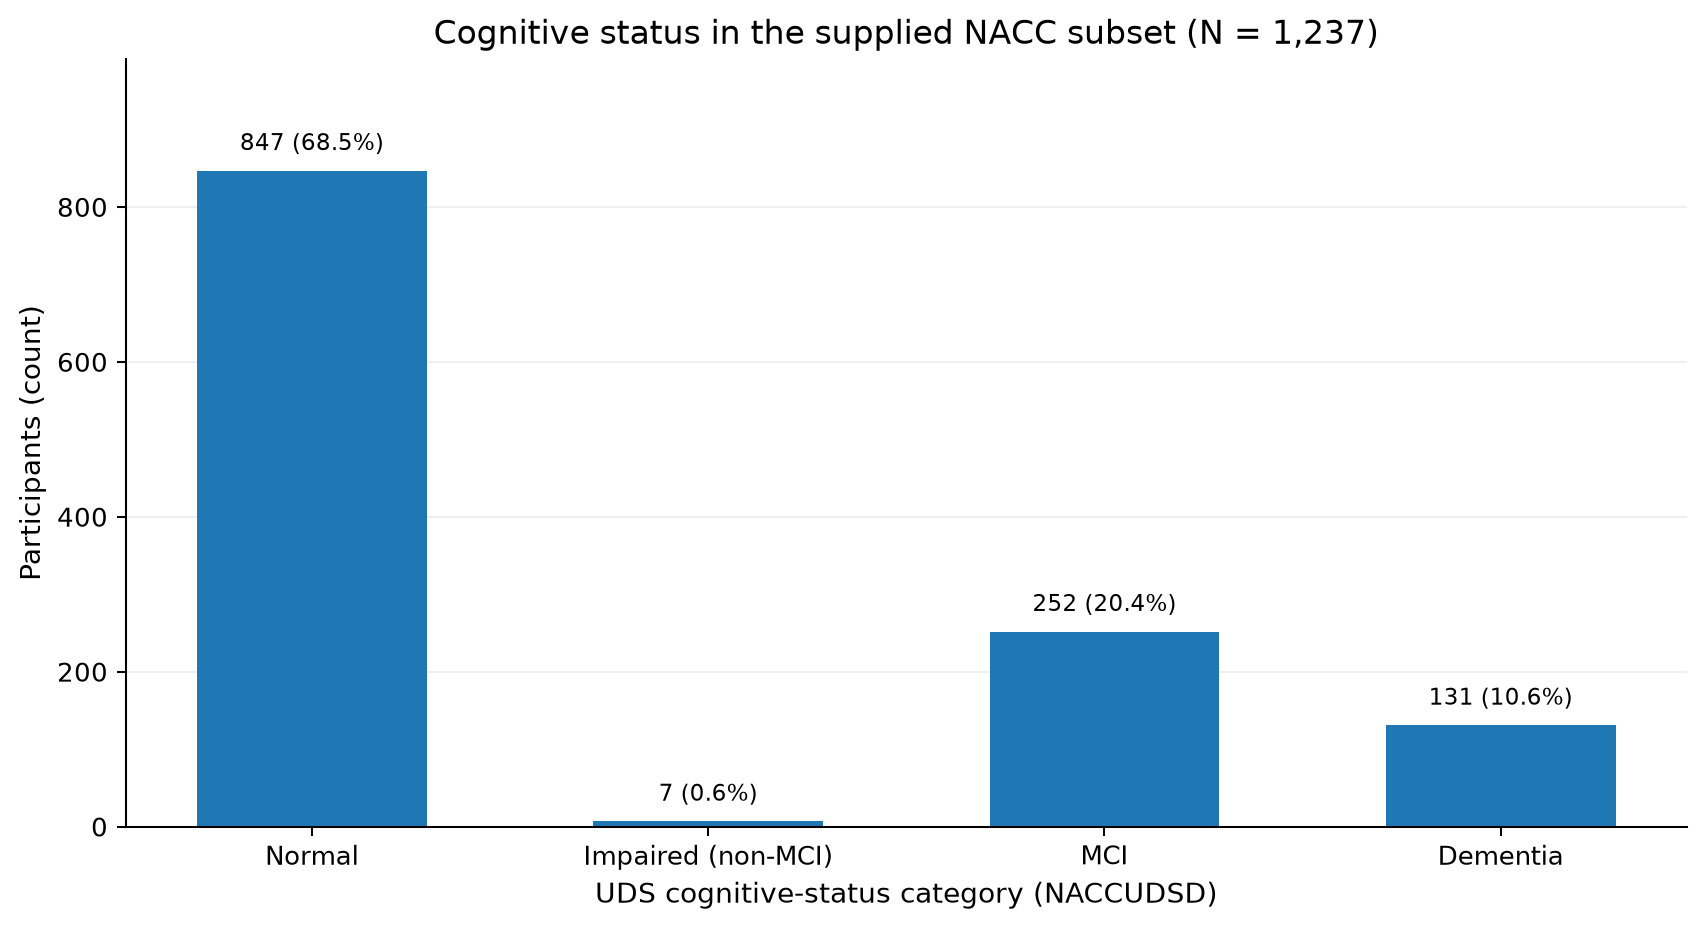
\includegraphics[width=.82\linewidth]{phase1_08_01_cognitive_group_counts.png}
\caption{فراوانی چهار گروه وضعیت شناختی در زیرمجموعه تحویلی؛ تفاوت اندازه گروه‌ها آشکار است.}
\end{figure}

\begin{figure}[H]\centering
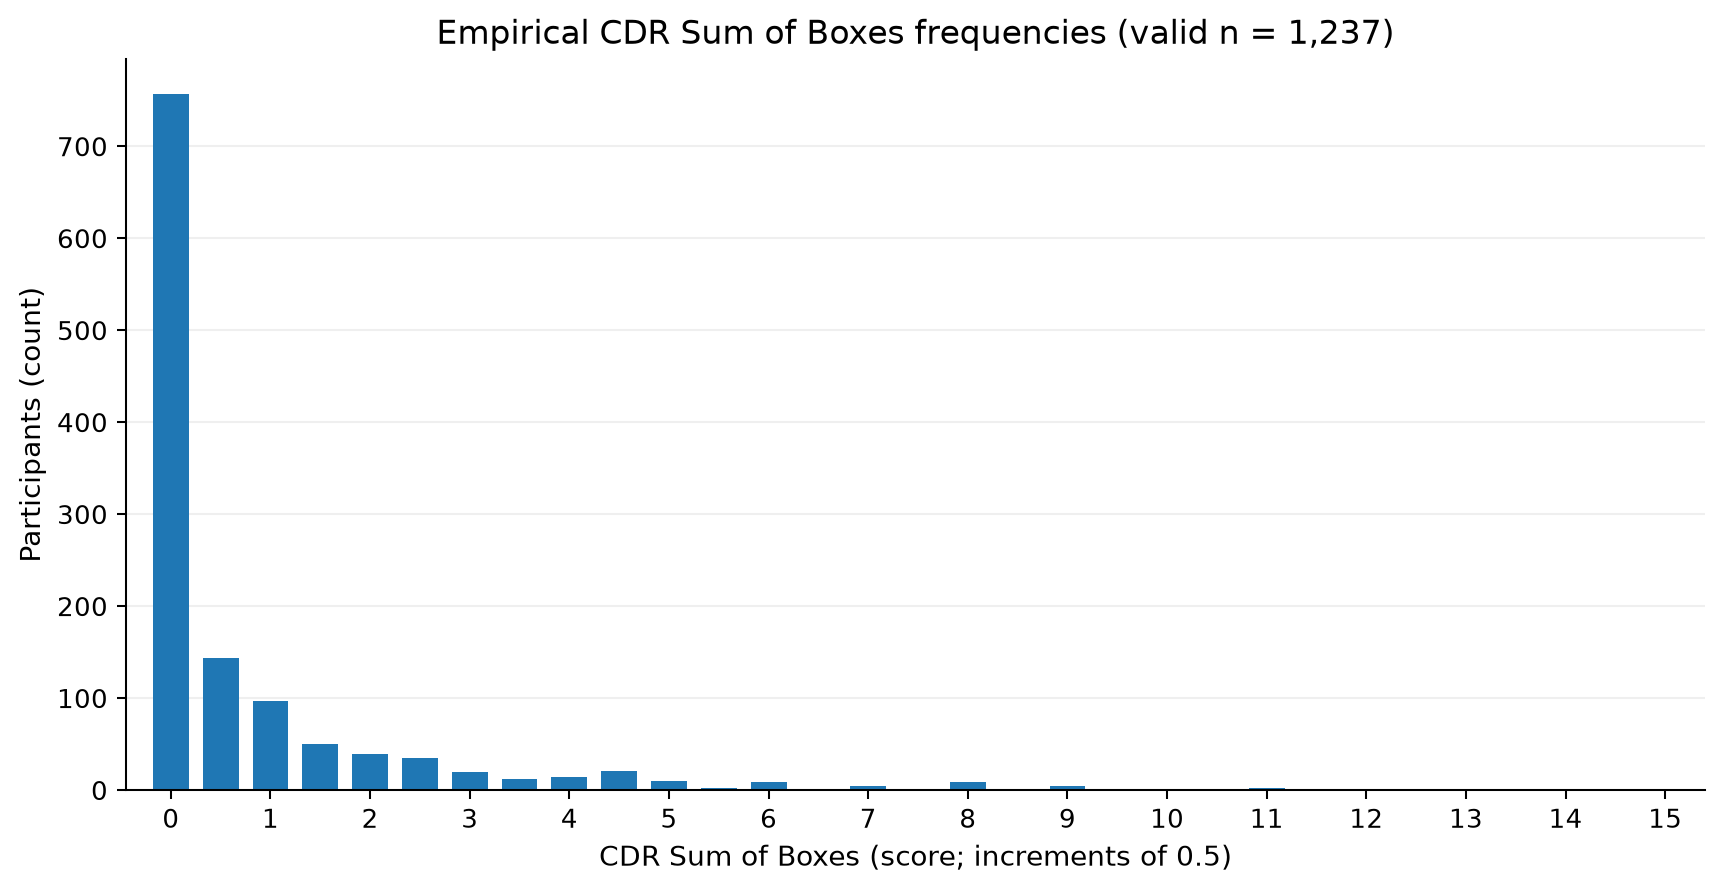
\includegraphics[width=.82\linewidth]{phase1_08_02_cdrsum_discrete_distribution.png}
\caption{فراوانی تجربی امتیاز نیم‌واحدی \Code{CDRSUM}؛ تمرکز روی صفر و دنباله راست.}
\end{figure}
\clearpage
\begin{figure}[H]\centering
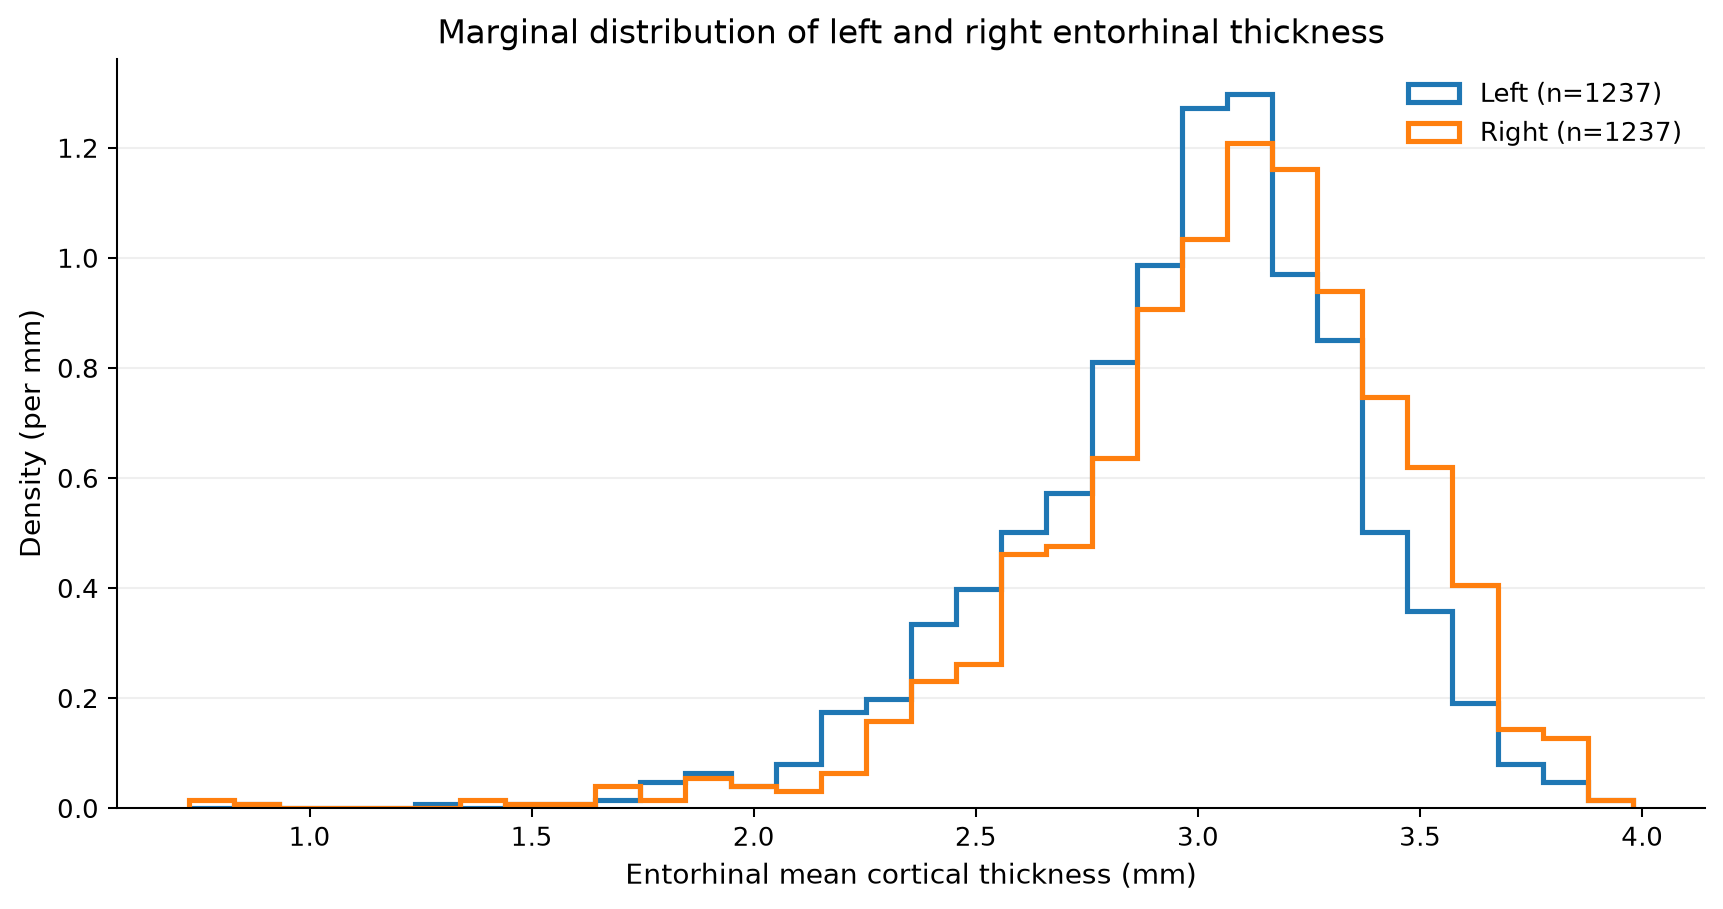
\includegraphics[width=.82\linewidth]{phase1_08_03_mri_thickness_distribution.png}
\caption{توزیع ضخامت انتورینال چپ و راست؛ محور افقی برحسب میلی‌متر و محور عمودی چگالی است.}
\end{figure}

\begin{figure}[H]\centering
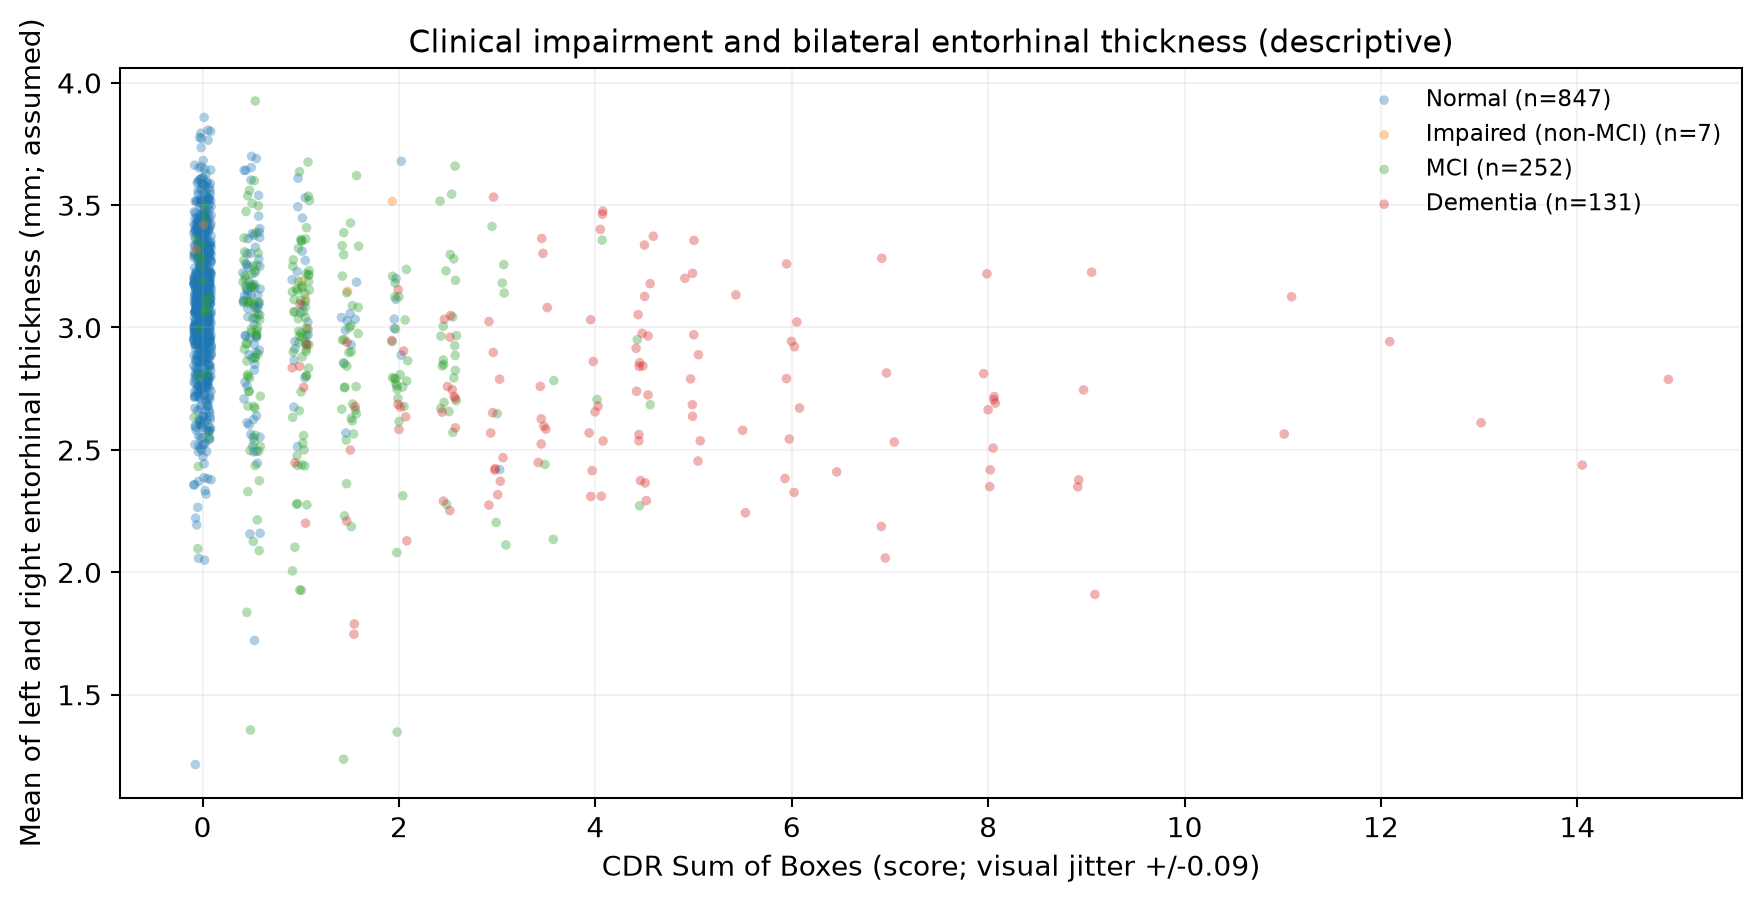
\includegraphics[width=.82\linewidth]{phase1_c5_joint_uds_mri_scatter.png}
\caption{نمایش جفت‌شده نمره بالینی UDS و میانگین ضخامت انتورینال دوطرفه MRI. رنگ‌ها گروه‌های شناختی‌اند؛ جابه‌جایی افقی تصادفی با بذر ثابت در بازه \En{$\pm0.09$} صرفا برای نمایش نقاط هم‌پوشان است و در محاسبات اعمال نشده است.}
\label{fig:joint-uds-mri}
\end{figure}
\textbf{دلیل انتخاب:} نمودار میله‌ای برای متغیر طبقه‌ای و نمره گسسته، هیستوگرام برای متغیر پیوسته
و نمودار پراکنش برای نمایش توصیفی دو وجه مناسب است. مقایسه گروه‌ها در بخش بعدی به کمک
جداول جداگانه انجام شده؛ در آن جداول تمام مقادیر، از جمله نقاط دورافتاده، حفظ شده‌اند.

\clearpage

\section{مقایسه توصیفی اولیه}
طبق سوال نهایی، چهار شاخص کمّی روی همان چهار گروه\,
\Code{NACCUDSD} مقایسه شده‌اند. همه خلاصه‌ها با اتصال یک‌به‌یک بر اساس
\Code{NACCID} محاسبه می‌شوند؛ هر شرکت‌کننده یک بار در هر جدول حضور دارد.
در جدول‌های زیر انحراف معیار با مخرج \En{$n-1$} و دامنه بین‌چارکی \En{$IQR=Q_3-Q_1$}
گزارش شده‌اند.
\Needspace{12\baselineskip}\subsection*{نمره بالینی CDRSUM (امتیاز)}
\small
\begin{longtable}{ p{3.5cm} r r r r r }
\toprule
گروه & تعداد & میانگین & میانه & انحراف معیار & IQR \\
\midrule
\endfirsthead
\toprule
گروه & تعداد & میانگین & میانه & انحراف معیار & IQR \\
\midrule
\endhead
شناخت طبیعی & 847 & 0.102 & 0.000 & 0.314 & 0.000 \\
اختلال شناختی غیر از MCI & 7 & 0.929 & 1.000 & 0.732 & 0.750 \\
اختلال شناختی خفیف (MCI) & 252 & 1.242 & 1.000 & 0.915 & 1.125 \\
دمانس & 131 & 4.664 & 4.500 & 2.711 & 3.000 \\
\bottomrule
\end{longtable}
\normalsize
\Needspace{12\baselineskip}\subsection*{ضخامت انتورینال چپ (میلی‌متر)}
\small
\begin{longtable}{ p{3.5cm} r r r r r }
\toprule
گروه & تعداد & میانگین & میانه & انحراف معیار & IQR \\
\midrule
\endfirsthead
\toprule
گروه & تعداد & میانگین & میانه & انحراف معیار & IQR \\
\midrule
\endhead
شناخت طبیعی & 847 & 3.046 & 3.069 & 0.336 & 0.402 \\
اختلال شناختی غیر از MCI & 7 & 3.156 & 3.260 & 0.347 & 0.239 \\
اختلال شناختی خفیف (MCI) & 252 & 2.863 & 2.920 & 0.432 & 0.569 \\
دمانس & 131 & 2.674 & 2.670 & 0.390 & 0.519 \\
\bottomrule
\end{longtable}
\normalsize
\Needspace{12\baselineskip}\subsection*{ضخامت انتورینال راست (میلی‌متر)}
\small
\begin{longtable}{ p{3.5cm} r r r r r }
\toprule
گروه & تعداد & میانگین & میانه & انحراف معیار & IQR \\
\midrule
\endfirsthead
\toprule
گروه & تعداد & میانگین & میانه & انحراف معیار & IQR \\
\midrule
\endhead
شناخت طبیعی & 847 & 3.132 & 3.150 & 0.338 & 0.415 \\
اختلال شناختی غیر از MCI & 7 & 3.330 & 3.376 & 0.192 & 0.263 \\
اختلال شناختی خفیف (MCI) & 252 & 2.953 & 3.014 & 0.493 & 0.509 \\
دمانس & 131 & 2.764 & 2.747 & 0.413 & 0.600 \\
\bottomrule
\end{longtable}
\normalsize
\Needspace{12\baselineskip}\subsection*{میانگین ضخامت انتورینال دوطرفه (میلی‌متر فرضی)}
\small
\begin{longtable}{ p{3.5cm} r r r r r }
\toprule
گروه & تعداد & میانگین & میانه & انحراف معیار & IQR \\
\midrule
\endfirsthead
\toprule
گروه & تعداد & میانگین & میانه & انحراف معیار & IQR \\
\midrule
\endhead
شناخت طبیعی & 847 & 3.089 & 3.103 & 0.304 & 0.369 \\
اختلال شناختی غیر از MCI & 7 & 3.243 & 3.188 & 0.182 & 0.236 \\
اختلال شناختی خفیف (MCI) & 252 & 2.908 & 2.966 & 0.413 & 0.500 \\
دمانس & 131 & 2.719 & 2.691 & 0.355 & 0.484 \\
\bottomrule
\end{longtable}
\normalsize

\Needspace{12\baselineskip}
\noindent\textbf{تفسیر مقایسه‌ای:}
در گروه شناخت طبیعی (۸۴۷ نفر)، میانه \Code{CDRSUM} برابر صفر است؛
در گروه \En{MCI} (۲۵۲ نفر) میانه برابر ۱ و در گروه دمانس (۱۳۱ نفر) برابر ۴٫۵ است.
در همین ترتیب، میانگین ضخامت انتورینال چپ از حدود ۳٫۰۴۶ به ۲٫۸۶۳
و ۲٫۶۷۴ میلی‌متر و میانگین سمت راست از حدود ۳٫۱۳۲ به ۲٫۹۵۳ و
۲٫۷۶۴ میلی‌متر تغییر می‌کند. این تفاوت‌ها فقط درباره زیرمجموعه درس صادق‌اند.
گروه اختلال غیر \En{MCI} تنها ۷ مشاهده دارد و مقادیر آن با نوسان نمونه‌ای
زیاد و بدون فرض ترتیب بالینی عددی کدهای گروه‌بندی تفسیر می‌شوند.

\section{نقشه کامل زیرمجموعه UDS و MRI}
\textbf{قلمرو:} دو فایل واقعی تحویلی تیم درس مبنای طبقه‌بندی هستند؛ کد \Code{NACCID}
شناسه فرد و \Code{NACCUDSD} برچسب وضعیت شناختی است.

\subsection*{طبقه‌بندی تمام ستون‌های UDS}
\small
\begin{longtable}{ p{11cm} r }
\toprule
خانواده متغیرها & تعداد ستون \\
\midrule
\endfirsthead
\toprule
خانواده متغیرها & تعداد ستون \\
\midrule
\endhead
آزمون‌های شناختی & 11 \\
امتیازهای CDR بالینی/عملکردی & 8 \\
اندازه‌گیری/معاینه بالینی & 14 \\
تشخیص/وضعیت شناختی & 1 \\
جمعیت‌شناختی/محیط زندگی & 9 \\
خانوادگی & 11 \\
رفتاری/روان‌پزشکی NPI-Q & 25 \\
سابقه پزشکی و روان‌پزشکی & 44 \\
شناسه/اتصال & 1 \\
عملکرد روزمره & 11 \\
محیط زندگی & 1 \\
محیط زندگی/عملکرد & 1 \\
مصرف دارو/سبک زندگی & 6 \\
پرسشنامه خلق GDS & 17 \\
گروه‌های دارویی & 20 \\
\bottomrule
\end{longtable}
\normalsize
فهرست تمام ۱۸۰ ستون با گروه و نقش در فایل
\path{data/derived/phase1/c123/c1_uds_variable_map.csv} قابل مشاهده و بازتولید است.
گروه‌های اصلی شامل جمعیت‌شناختی و زندگی، سابقه پزشکی و خانوادگی، مصرف دارو،
عملکرد روزمره، خلق و رفتار، آزمون‌های شناختی و نمره‌های \En{CDR} هستند.
در سوال نهایی، \Code{CDRSUM} متغیر توضیحی، میانگین ضخامت دوطرفه پاسخ اصلی و \Code{NACCUDSD} گروه‌بندی توصیفی است.

\subsection*{معنای ۱۲۴ ویژگی MRI}
\textbf{الگوی نام‌گذاری:} پیشوند \Code{LH} نیمکره چپ، \Code{RH} نیمکره راست؛
پسوند \Code{AVGTH} «میانگین ضخامت قشر ناحیه» (میلی‌متر در گزارش درس) و
پسوند \Code{GVOL} «حجم ماده خاکستری همان ناحیه» است. واحد خام ستون‌های حجمی
و نوع پردازش و نسخه اطلس از فایل‌ها قابل احراز نیست؛ هیچ واحد حجمی حدسی ثبت نشده است.
\Code{NACCUDSD} در فایل MRI یک برچسب بالینی است، نه اندازه‌گیری مستقل تصویری.
\small
\begin{longtable}{ p{11cm} r }
\toprule
نوع ستون MRI & تعداد \\
\midrule
\endfirsthead
\toprule
نوع ستون MRI & تعداد \\
\midrule
\endhead
ویژگی حجمی ناحیه‌ای، دو نیمکره & 62 \\
میانگین ضخامت قشر ناحیه‌ای، دو نیمکره & 62 \\
شناسه و برچسب شناختی (نه ویژگی تصویر) & 2 \\
جمع & 126 \\
\bottomrule
\end{longtable}
\normalsize
۳۱ ناحیه MRI (هرکدام در دو نیمکره و با دو نوع اندازه‌گیری):
\small
\begin{longtable}{ p{7cm} p{7cm} }
\toprule
ناحیه & ناحیه \\
\midrule
\endfirsthead
\toprule
ناحیه & ناحیه \\
\midrule
\endhead
\En{caudal anterior cingulate} & \En{pars opercularis} \\
\En{caudal middle frontal} & \En{pars orbitalis} \\
\En{cuneus} & \En{pars triangularis} \\
\En{entorhinal cortex} & \En{pericalcarine cortex} \\
\En{fusiform gyrus} & \En{postcentral cortex} \\
\En{inferior parietal cortex} & \En{posterior cingulate cortex} \\
\En{inferior temporal cortex} & \En{precentral cortex} \\
\En{insula} & \En{precuneus} \\
\En{isthmus cingulate} & \En{rostral anterior cingulate} \\
\En{lateral occipital cortex} & \En{rostral middle frontal} \\
\En{lateral orbitofrontal cortex} & \En{superior frontal cortex} \\
\En{lingual gyrus} & \En{superior parietal cortex} \\
\En{medial orbitofrontal cortex} & \En{superior temporal cortex} \\
\En{middle temporal cortex} & \En{supramarginal gyrus} \\
\En{paracentral cortex} & \En{transverse temporal cortex} \\
\En{parahippocampal cortex} &  \\
\bottomrule
\end{longtable}
\normalsize
فایل \Code{c1_mri_variable_map.csv} در پوشه \Code{data/derived/phase1/c123/}
برای تمام ۱۲۶ ستون MRI نام ناحیه، نیمکره، نوع اندازه‌گیری و واحد معلوم یا نامشخص را جداگانه ثبت می‌کند.
دو ستون مورد استفاده این پروژه، \Code{LH_ENTORHINAL_AVGTH} و
\Code{RH_ENTORHINAL_AVGTH}، میانگین ضخامت قشر انتورینال چپ و راست‌اند.
ماتریس مجاورت ۶۲ ناحیه نیز در موجودی‌گیری ثبت شده اما متغیرهای پاسخ این پرسش را نمی‌سازد.

\section{ساختار شرکت‌کننده و مراجعه}
در پایگاه کامل \En{NACC}، \En{UDS} عموما ساختار طولی دارد و یک ردیف
می‌تواند نماینده یک مراجعه یک فرد باشد؛ اما در زیرمجموعه درسی کنونی
هر فرد در هر فایل دقیقا یک ردیف دارد. این شمارش به معنی آن نیست که
هر فرد در پایگاه اصلی فقط یک مراجعه داشته است.
\small
\begin{longtable}{ p{3.2cm} p{7.5cm} r }
\toprule
فایل & تعداد سطر هر فرد در فایل تحویلی & تعداد افراد \\
\midrule
\endfirsthead
\toprule
فایل & تعداد سطر هر فرد در فایل تحویلی & تعداد افراد \\
\midrule
\endhead
\En{UDS} & 1 & 1237 \\
\En{MRI} & 1 & 1237 \\
\bottomrule
\end{longtable}
\normalsize
\textbf{فراداده غایب:} ستون‌های شماره یا شمار مراجعات
\Code{NACCVNUM}، \Code{NACCAVST}، \Code{NACCNVST}، تاریخ ارزیابی
\Code{VISITMO}، \Code{VISITDAY}، \Code{VISITYR} و تاریخ‌های
اسکن مانند \Code{MRIYR} و \Code{MRIMO} در فایل‌های تحویلی وجود ندارند.
پس تعداد واقعی مراجعات و توزیع آن قابل برآورد از این فایل‌ها نیست.

\textbf{قاعده مشاهده شاخص:} برای فازهای بعدی فقط همان یک سطر تحویلی از
\En{UDS} و یک سطر از \En{MRI} به‌ازای هر \Code{NACCID}
استفاده می‌شود. این یک قاعده استفاده از زیرمجموعه آماده است، نه
قاعده تازه برای انتخاب آخرین یا اولین مراجعه واقعی. هر فرد یک مشاهده مستقل
در سطح شناسه خواهد بود؛ ادعایی درباره هم‌زمانی اسکن و معاینه نداریم.

\section{اتصال یک‌به‌یک UDS و MRI}
اتصال بر اساس \Code{NACCID} و پس از کنترل یکتایی و تهی نبودن شناسه
انجام شده است. کد اگر شناسه تکراری ببیند، به‌جای ساختن اتصال چندبه‌چند
و چندبار شمردن فرد، با خطا متوقف می‌شود. کدهای \Code{NACCUDSD}
در دو فایل به شکل عددی هم‌معنا مقایسه شده‌اند؛ به‌عنوان مثال \En{1.0}
در فایل UDS با \En{1} در MRI یک طبقه است و عدم تطابق واقعی نیست.
\small
\begin{longtable}{ p{11cm} r }
\toprule
مرحله اتصال & تعداد \\
\midrule
\endfirsthead
\toprule
مرحله اتصال & تعداد \\
\midrule
\endhead
سطرهای خام UDS & 1237 \\
شرکت‌کنندگان یکتای UDS & 1237 \\
سطرهای خام MRI & 1237 \\
شرکت‌کنندگان یکتای MRI & 1237 \\
شرکت‌کنندگان مشترک & 1237 \\
فقط UDS & 0 \\
فقط MRI & 0 \\
ردیف‌های اتصال نهایی یک‌به‌یک & 1237 \\
اختلاف واقعی کد وضعیت شناختی & 0 \\
سطرهای دارای پنج ستون کنترل‌شده غیرخالی & 1237 \\
\bottomrule
\end{longtable}
\normalsize

\textbf{محدودیت زمانی:} راهنمای رسمی \En{NACC} صریح می‌گوید اسکن‌ها
لزومی ندارد با همان مراجعه \En{UDS} ثبت شده باشند. نبودن تاریخ‌ها در
زیرمجموعه ما مانع کنترل فاصله زمانی و تطبیق مراجعه بالینی با اسکن است.

\textbf{فایل‌های بازتولیدپذیر:} همه جدول‌های تجمیعی سه تسک ویژه در
\Code{data/derived/phase1/c123/} قرار می‌گیرند و هیچ شناسه واقعیِ فرد در این
جدول‌ها صادر نمی‌شود. برای اجرای دوباره، اسکریپت
\Code{src/06_subset_structure_merge.py} همراه اجرای اصلی استفاده می‌شود.

\section{گمشدگی و انتخاب نمونه چندوجهی}
\textbf{تعریف سه نوع وضعیت:} نخست «خانه واقعا خالی در CSV تحویلی»،
دوم «کد ویژه نامعتبر برای تحلیل همان متغیر» مطابق نگاشت متغیر-ویژه،
و سوم «مقدار قابل پرچم‌گذاری برای کنترل کیفیت» جداگانه شمارش شده‌اند.
این سه وضعیت نباید با هم جمع بسته و بدون توضیح «داده گمشده اولیه» نامیده شوند.
\subsection*{درصد گمشدگی در متغیرهای منتخب هر دو وجه}
\small
\begin{longtable}{ p{5.0cm} r r r r r }
\toprule
وجه / متغیر & خالی خام & درصد خام & کد ویژه & پرچم کیفیت & معتبر \\
\midrule
\endfirsthead
\toprule
وجه / متغیر & خالی خام & درصد خام & کد ویژه & پرچم کیفیت & معتبر \\
\midrule
\endhead
\Code{NACCUDSD} & 0 & 0.0 & 0 & 0 & 1237 \\
\Code{CDRSUM} & 0 & 0.0 & 0 & 0 & 1237 \\
\Code{NACCAGE} & 0 & 0.0 & 0 & 0 & 1237 \\
\Code{SEX} & 0 & 0.0 & 0 & 0 & 1237 \\
\Code{EDUC} & 0 & 0.0 & 2 & 0 & 1235 \\
\Code{MOCATOTS} & 0 & 0.0 & 4 & 249 & 984 \\
\Code{LH_ENTORHINAL_AVGTH} & 0 & 0.0 & 0 & 0 & 1237 \\
\Code{RH_ENTORHINAL_AVGTH} & 0 & 0.0 & 0 & 0 & 1237 \\
\bottomrule
\end{longtable}
\normalsize

\textbf{یافته‌های متغیر-ویژه:} در \Code{EDUC} تعداد 2
رکورد با کد \En{99} و در \Code{MOCATOTS} تعداد 4
رکورد با کد \En{88} یا \En{-4} قابل استفاده به‌عنوان مقدار نمره نیستند.
برای \Code{MOCATOTS} تعداد 5
مقدار خارج از دامنه نمره و 249 مقدار اعشاری
به‌عنوان پرچم کیفیت ثبت شده‌اند (این دو دسته می‌توانند همپوشانی داشته باشند).
با توجه به نام \En{imputed} فایل، این مقادیر خودکار اصلاح یا گرد نشده‌اند و
تا روشن‌شدن روش جایگذاری، در آمار نمره MoCA استفاده نمی‌شوند.
در مقابل چهار شاخص اصلی سوال، \Code{CDRSUM} و ضخامت انتورینال چپ و راست،
در فایل تحویلی برای تمام افراد مقدار عددی و در بازه کنترل‌شده دارند.

\subsection*{پوشش MRI و عدم امکان مقایسه «دارای / فاقد MRI»}
\small
\begin{longtable}{ p{11cm} r }
\toprule
معیار پوشش & تعداد \\
\midrule
\endfirsthead
\toprule
معیار پوشش & تعداد \\
\midrule
\endhead
افراد UDS دارای رکورد MRI & 1237 \\
افراد UDS بدون رکورد MRI در فایل تحویلی & 0 \\
ستون ویژگی واقعی MRI بررسی‌شده & 124 \\
خانه خالی در همه ویژگی‌های MRI & 0 \\
مقادیر غیرمثبت در ویژگی‌های MRI: پرچم کنترل کیفیت & 2 \\
\bottomrule
\end{longtable}
\normalsize

تمام افراد \En{UDS} در این زیرمجموعه آماده یک رکورد MRI دارند.
بنابراین شاخص «داشتن MRI» ثابت و مقایسه توصیفی افراد دارای MRI با
فاقد MRI در این فایل ناممکن است؛ از داده‌های موجود نمی‌توان
درباره انتخاب‌شدن برای اسکن در کل پایگاه NACC نتیجه گرفت.
برای توصیف گروه موجود، فراوانی‌های کدهای شناختی UDS در افراد دارای MRI ثبت شدند:
\small
\begin{longtable}{ p{8.0cm} r r }
\toprule
کد وضعیت شناختی & تعداد & درصد \\
\midrule
\endfirsthead
\toprule
کد وضعیت شناختی & تعداد & درصد \\
\midrule
\endhead
1 & 847 & 68.5 \\
2 & 7 & 0.6 \\
3 & 252 & 20.4 \\
4 & 131 & 10.6 \\
\bottomrule
\end{longtable}
\normalsize

در همان زیرنمونه دارای MRI، میانگین سن 68.19 سال
و میانگین \Code{CDRSUM} برابر 0.822 است.
این خلاصه‌ها یک گروه موجود را توصیف می‌کنند؛ جدول مقایسه دو گروه نیستند.
تعداد 2 مقدار غیرمثبت در کل ۱۲۴ ستون
MRI صرفا پرچم کنترل کیفیت است: بدون شرح پردازش تصویر، صفر را
به‌صورت خودکار «گمشده» یا خطای قطعی فرض نمی‌کنیم. این دو مورد به دو
شاخص ضخامت انتورینال منتخب مربوط نیستند. هیچ رکوردی به این دلیل حذف نشده است.

\section{خلاصه مشترک شناختی و تصویربرداری}
شرکت‌کنندگان با کلید \Code{NACCID} و فقط یک مشاهده تحویلی از هر وجه
به‌صورت یک‌به‌یک هم‌تراز شدند. در زیرمجموعه مشترک 1237 نفر
دارای \Code{CDRSUM} معتبر از UDS و دو ضخامت انتورینال معتبر از MRI هستند؛ شاخص دوطرفه از میانگین همان دو مقدار ساخته شد؛
تعداد رکوردهای کنارگذاشته‌شده به‌علت نبود/نامعتبربودن این چهار شاخص برابر
0 است.

\subsection*{خلاصه توزیع چهار شاخص در افراد مشترک}
\small
\begin{longtable}{ p{3.5cm} r r r r p{2.3cm} r }
\toprule
متغیر & میانگین & میانه & انحراف معیار & IQR & دامنه & پرت IQR \\
\midrule
\endfirsthead
\toprule
متغیر & میانگین & میانه & انحراف معیار & IQR & دامنه & پرت IQR \\
\midrule
\endhead
امتیاز بالینی CDRSUM & 0.822 & 0.000 & 1.723 & 1.000 & 0.000 تا 15.000 & 115 \\
ضخامت انتورینال چپ (mm) & 2.970 & 3.021 & 0.384 & 0.465 & 0.878 تا 3.979 & 28 \\
ضخامت انتورینال راست (mm) & 3.058 & 3.097 & 0.401 & 0.466 & 0.729 تا 3.967 & 30 \\
میانگین دوطرفه (mm؛ فرضی) & 3.014 & 3.058 & 0.356 & 0.449 & 1.214 تا 3.925 & 22 \\
\bottomrule
\end{longtable}
\normalsize

\textbf{روش:} انحراف معیار با مخرج \En{$n-1$}، چارک‌ها با درون‌یابی خطی
و نقاط پرت با حصارهای \En{$Q_1-1.5IQR$} و \En{$Q_3+1.5IQR$}
محاسبه شده‌اند. موارد بیرون از حصار صرفا توصیف شده و در میانگین و نمودارها
باقی مانده‌اند؛ به‌ویژه تراکم \Code{CDRSUM} روی صفر باعث می‌شود این قاعده
برای این امتیاز صرفا یک شاخص توصیفی، نه ملاک غیرعادی‌بودن بالینی، باشد.

\subsection*{خلاصه گروهی هم‌تراز بین UDS و MRI}
\small
\begin{longtable}{ p{4.1cm} r r r r }
\toprule
گروه شناختی & تعداد & میانه CDRSUM & میانگین دوطرفه & انحراف معیار دوطرفه \\
\midrule
\endfirsthead
\toprule
گروه شناختی & تعداد & میانه CDRSUM & میانگین دوطرفه & انحراف معیار دوطرفه \\
\midrule
\endhead
شناخت طبیعی & 847 & 0.000 & 3.089 & 0.304 \\
اختلال شناختی غیر از MCI & 7 & 1.000 & 3.243 & 0.182 \\
اختلال شناختی خفیف (MCI) & 252 & 1.000 & 2.908 & 0.413 \\
دمانس & 131 & 4.500 & 2.719 & 0.355 \\
\bottomrule
\end{longtable}
\normalsize

نمودار چهارم (شکل \ref{fig:joint-uds-mri}) جفت‌های نمره بالینی و ضخامت دوطرفه را
همراه جدول‌های این بخش نمایش می‌دهد.

\section{نهایی‌سازی سوال آماری و تناسب داده}
\textbf{سوال نهایی:} آیا نمره \Code{CDRSUM} با میانگین ضخامت قشر انتورینال چپ و راست مرتبط است و این ارتباط با درنظرگرفتن سن و جنس چگونه تغییر می‌کند؟ متغیر پاسخ اصلی \Code{ENTORHINAL_MEAN_AVGTH} و توضیحی اصلی \Code{CDRSUM} است. سن و جنس فقط برای تحلیل‌های مراحل بعدی معرفی شده‌اند و در فاز اول هیچ مدل تعدیل‌شده‌ای برازش نشده است.

\textbf{تناسب داده:} 1237 شرکت‌کننده یکتا در هر دو وجه \En{UDS} و \En{MRI} ثبت شده‌اند. طبق جدول‌های قابل بازتولید، هر 1237 نفر در \Code{CDRSUM} و هر دو ستون ضخامت انتورینال مقدار معتبر دارند. میانگین ضخامت دوطرفه برای هر فرد از همین دو ستون ساخته شده است. میانگین نمونه‌ای آن 3.014 و انحراف معیار نمونه‌ای 0.356 است (واحد میلی‌متر فرض شده است). نمودار چهارم نمایش توصیفی جفت‌های واقعی را فراهم می‌کند.

\textbf{دامنه و محدودیت:} این زیرمجموعه نماینده جامعه عمومی نیست؛ تاریخ اسکن و مراجعه، فرایند انتخاب نمونه و روش جایگذاری UDS در فایل‌ها مشخص نشده‌اند. رابطه مشاهده‌ای دلیل بر علیت یا هم‌زمانی نیست. مقایسه تعدیل‌شده بر حسب سن و جنس، آزمون فرض، فاصله اطمینان و رگرسیون موضوع فاز اول نیستند.

\section{روش بازتولید و مراجع}
\textbf{داده خام:} سه CSV تحویلی در \Code{data/raw/} قرار دارند و اسکریپت‌ها
آن‌ها را تغییر نمی‌دهند. برای اجرای کامل بخش انجام‌شده، از ریشه مخزن:
\begin{latin}
\begin{verbatim}
python -m pip install -r requirements.txt
python src/run_phase1.py
\end{verbatim}
\end{latin}
نسخه قابل بازتولید گزارش در \Code{reports/phase1.tex} نوشته می‌شود.

فایل‌های ممیزی ریزدانه که ممکن است دارای شناسه \Code{NACCID} باشند،
فقط به‌صورت محلی در \Code{data/derived/} ذخیره می‌شوند.
این پوشه با \Code{.gitignore} از انتشار کنار گذاشته شده است.
برای نمایش چهار نمودارِ گزارش، به چهار فایل PNG در پوشه \Code{figures/} نیاز است.
جداول محاسباتی در پوشه \Code{data/derived/phase1/} ساخته می‌شوند.
گزارش با \En{XeLaTeX} قابل بازتولید است.

\textbf{مراجع اصلی:}
\begin{enumerate}
\item دستورالعمل رسمی تیم دستیاری، \Code{docs/amarpr.pdf}
\item \href{https://www.naccdata.org/about-nacc-data}{\En{NACC -- About NACC Data}}.
\item \href{https://www.naccdata.org/data-forms-and-documentation/}{\En{NACC -- Data Forms and Documentation}}.
\item \href{https://www.naccdata.org/the-nacc-researchers-guide}{\En{NACC -- The Researcher's Guide}}.
\end{enumerate}

\end{document}
